\documentclass[tikz,border=5pt,multi=tikzpicture]{standalone}
\usepackage[UTF8]{ctex}
\usepackage{amsmath}
\usetikzlibrary{arrows.meta,calc}
\definecolor{ink}{HTML}{17365D}
\definecolor{field}{HTML}{287DA8}
\definecolor{force}{HTML}{C56B2A}
\tikzset{every node/.style={font=\small},vec/.style={-{Stealth[length=2mm]},thick},helper/.style={gray,dashed}}
\begin{document}
\begin{tikzpicture}
  \coordinate (O) at (0,0);\coordinate (Ob) at (.16,.11);
  \coordinate (P1) at (-1.1,-.55);\coordinate (P2) at (1.26,.66);
  \filldraw[gray!65,fill=gray!10] (-1.64,-1.59)--(1.96,-.34)--(1.96,1.81)--(-1.64,.56)--cycle;
  \filldraw[gray!75,fill=gray!4] (-1.8,-1.7)--(1.8,-.45)--(1.8,1.7)--(-1.8,.45)--cycle;
  \draw[gray!65] (-1.8,-1.7)--(-1.64,-1.59);
  \draw[gray!65] (1.8,-.45)--(1.96,-.34);
  \draw[gray!65] (1.8,1.7)--(1.96,1.81);
  \draw[gray!65] (-1.8,.45)--(-1.64,.56);
  \draw[helper,thick] (Ob)--(P2) node[midway,above left] {$l$};
  \draw[gray,dashed,fill=white] (P2) circle (.10) node[above right] {$m$};
  \draw[helper] (O)--(Ob);
  \draw[ink,thick,fill=white] (O) ellipse (.08 and .105);
  \draw[ink,very thick] (O)--(P1) node[midway,below right] {$l$};
  \filldraw[ink,fill=white] (P1) circle (.10) node[below left] {$m$};
  \node[above left,xshift=-3pt] at (O) {$O$};
  \draw[vec,force] (215:1.42) arc (215:270:1.42) node[midway,below left] {$\omega$};
  \draw[vec,gray] ($(Ob)+(35:1.42)$) arc (35:85:1.42) node[midway,right] {$\omega$};
  \node[ink] at (-.7,-.95) {板前};
  \node[gray] at (2.55,1.05) {板后};
\end{tikzpicture}
\begin{tikzpicture}
  \foreach \j/\shift/\radius/\radiuslabel in {1/0/1.65/{r_1=l+x},2/5.1/.85/{r_2=l-x}}{
    \begin{scope}[xshift=\shift cm]
      \draw[helper] (0,0) circle (1.25);
      \draw[field,thin] (0,0) circle (\radius);
      \draw[field,thick] (0,0)--(\radius,0) node[midway,below] {$\radiuslabel$};
      \fill (0,0) circle (1.4pt) node[above left] {$O$};
      \filldraw[ink,fill=white] (\radius,0) circle (.075) node[right,xshift=3pt] {$m$};
      \draw[vec,force] (35:{\radius+.2}) arc (35:95:{\radius+.2}) node[midway,above] {$\dot\theta_\j$};
      \node at (0,-2.05) {第 $\j$ 侧};
    \end{scope}
  }
\end{tikzpicture}
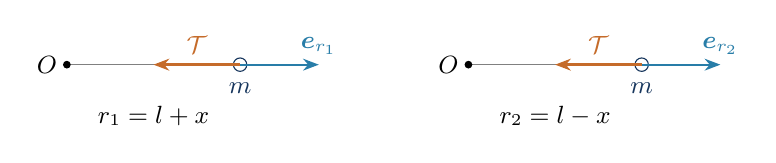
\begin{tikzpicture}
  \foreach \j/\shift/\radius in {1/0/{l+x},2/5.1/{l-x}}{
    \begin{scope}[xshift=\shift cm]
      \draw[gray] (0,0)--(2.2,0);
      \fill (0,0) circle (1.4pt) node[left] {$O$};
      \filldraw[ink,fill=white] (2.2,0) circle (.085) node[below,yshift=-3pt] {$m$};
      \draw[vec,force,line width=1.1pt] (2.2,0)--(1.1,0) node[midway,above] {$\mathcal T$};
      \draw[vec,field] (2.2,0)--(3.2,0) node[above] {$\boldsymbol e_{r_\j}$};
      \node at (1.1,-.65) {$r_\j=\radius$};
    \end{scope}
  }
\end{tikzpicture}
\begin{tikzpicture}[x=4.5cm,y=.55cm]
  \draw[vec,gray] (-.79,0)--(.84,0) node[right] {$x/l$};
  \draw[vec,gray] (0,0)--(0,6.3) node[above] {$U_{\mathrm{eff}}/(m\omega^2l^2)$};
  \foreach \s/\ticklabel in {-.6/{-0.6},.6/{0.6}}{\draw (\s,.08)--(\s,-.08) node[below] {$\ticklabel$};}
  \foreach \u in {1,3,5}{\draw (.015,\u)--(-.015,\u) node[left,xshift=-2pt] {$\u$};}
  \draw[field,thick,domain=-.7:.7,samples=101] plot (\x,{(1+\x*\x)/(1-\x*\x)^2});
  \draw[force,thick,dashed,domain=-.7:.7,samples=61] plot (\x,{1+3*\x*\x});
  \fill[field] (0,1) circle (.015);
  \draw[field,thick] (-.58,5.6)--(-.45,5.6) node[right] {精确有效势};
  \draw[force,thick,dashed] (-.58,4.75)--(-.45,4.75) node[right] {二次近似};
\end{tikzpicture}
\end{document}
